\externaldocument{tech_eclipse_text}

\section{The Model \label{terminology}}
The eclipse mapping program described in this paper derives a model for the relative two-dimensional surface brightness of a transiting planet host star that matches an observed one-dimensional light curve of its integrated flux. We derive the brightness values for a set of discrete regions on the star as shown in Figure~\ref{bright_map} \citep{Huber2009}. Each iteration of the program produces a static map in which brightness values less than one correspond to regions of the star that contain starspots.  By applying the code to a series of short segments of the light curve, we are able to extract information about the time evolution of the star's surface brightness as described in \citet{Huber2010}. 

\subsection{Set-up and Terminology}

In order to efficiently describe the details of our program, the geometry of the problem must be defined and some basic terminology must be established. The star is assumed to be a uniformly rotating,  solid body with a single planet on a nearly circular orbit that periodically transits the star. The stellar surface is divided into a series of large regions, as shown in Figure~\ref{bright_map}.  While describing our program in this paper, the regions along the line of transit will be called {\it boxes}; the total longitudinal regions will be called {\it longitudes}; and the longitudinal regions with the {\it box} areas subtracted will be referred to as {\it stripes}. When talked about as an ensemble or when the distinction is unimportant, these regions will be referred to as just that - {\it regions}.The resolution of our brightness map is set by two parameters, the number of {\it boxes}, $n_b$, and  the number of stripes, $n_s$.  All of the {\it stripes} are the same size, and likewise so are the {\it boxes}. The width of each {\it stripe} (or {\it box}) is defined so that $n_s$ (or $n_b$) regions exactly covers the full $360^{\circ}$ stellar surface. The desnity of {\it boxes} is higher than that of the {\it stripes} because there is more information contained in the transit portions of the light curve. The number of {\it boxes}, $n_b$, is typically set to be an integer multiple of the number of {\it stripes} so that the boundaries of each longitude will always contain an integer number of {\it boxes}. 

The program takes a single-band, high-cadence light curve of a transiting planet host star along with its rotation period ($P_{rot}$) as inputs. Deriving a realistic brightness map also depends on including a precise model of the transit, thus certain physical properties of the star and the planet must be provided. The following parameters are used to produce the detailed transiting planet model: orbital period ($P_{orb}$), orbital separation ($a$), impact parameter ($b$), relative radius of the planet compared to the star ($\frac{R_p}{R^{*}}$), and two quadratic limb-darkening coefficients. Finally, the configuration of our {\it regions} requires that the spin-axis of the star is aligned with the orbital axis of the planet. *************** Ask Leslie for a line (Many stars aligned citation) ****** These criteria are both met for our test object, Kepler-17 \citep{Borucki2011}. %Cite the Desert 2011 RM measurements ****************

\begin{figure}[h]
	\centering
	\includegraphics[width=.5\textwidth]{images/model_map.eps}
	\caption{Recovered surface brightness map from our eclipse mapping program when using a simulated light curve with one dark spot group placed in the path of the planet. The figure shows the geometric set-up of a star that we are modeling. The {\it regions} approximately along the equator are in the path of the planet and are called {\it boxes}. Those out of the path of the planet are called {\it stripes}. In this case, the surface of the star is divided into 11 {\it stripes} and 22 {\it boxes}. Each stripe is $32.72^{\circ}$ and each box is $16.36^{\circ}$. In this simulation, we recover relative brightness values of approximately one everywhere except for the visibily darkened {\it box} which corresponds to a brighness value of 0.90.}
	\label{bright_map}
\end{figure}

In order to derive a discrete, two-dimensional brightness map that best reproduces the input light curve, the program calculates a model light curve by integrating over the surface of the visible sphere at each timestep according to:

\begin{equation}
	\fmod = \sum_j V_{i,j}b_j
\end{equation}

The model flux includes $b_j$, the brightness per unit area for {\it region} $j$ and $V_{i,j}$, the {\it visibility} of {\it region} $j$ at time, $i$. As the star rotates, the brightness of a {\it region}  does not change but its contribution to the total flux does. The amount of flux from each {\it region} that reaches the observer varies predictably and is captured in its visibility. Here, visibility is a measure of projected surface area along the line of sight to the observer. The transit by the planet also modifies the amount of flux that reaches the observer. Therefore, the area of the star blocked by the planet is explicitly included in the visibility calculations. The transit is accounted for by subtracting the area that the planet obscures of a given {\it box} from the normal visibility of the same {\it box} at each time step. It is important to include limb-darkening, which has a significant effect on the shape of the transit. We incorporate the quadratic limb-darkening law provided in \citet{Claret2004}.


%%The longitude values from equation~\ref{z_val} create parameter independence by changing the way that our algorithm navigates the chi-squared space so that such a case is less likely to become a local minimum. The Amoeba algorithm takes the set of box brightness guesses and longitude brightness guesses as inputs. During each call of the chi-squared algorithm the stripe values are calculated from the longitudes and boxes. The boxes and the stripes are then used to calculate the model flux.
%
%%Possibly move this next paragraph or restructure it. 
%Other inputs to the code include the binning cadence for both in and out-of-transit points of the light curve, the number of boxes ($n_b$) and stripes ($n_s$) there should be in the surface map, number of days per individual brightness solution or {\it window}, and the number of days to increment each window. In Figure~\ref{LC_Fit}, the window is the section with the red points.
%
%The data is binned according to two separate binning cadences. In-transit points give information about smaller scale features, so they are binned at a high cadence. The out-of-transit points are binned at a low cadence because the overall longterm variability of a longitude can be tracked well with less information. Added benefits of binning the out-of-transit points at a low cadence are that the run-time of the code decreases with fewer points to match in the light curve and there is some degree of inherent noise removal by binning. Care must be taken at the boundaries of in- and out-of-transit regions of the light curve. Some bins will be cut off with fewer points in order to properly switch between the two different binning cadences.
%\begin{figure}[h]
%	\centering
%	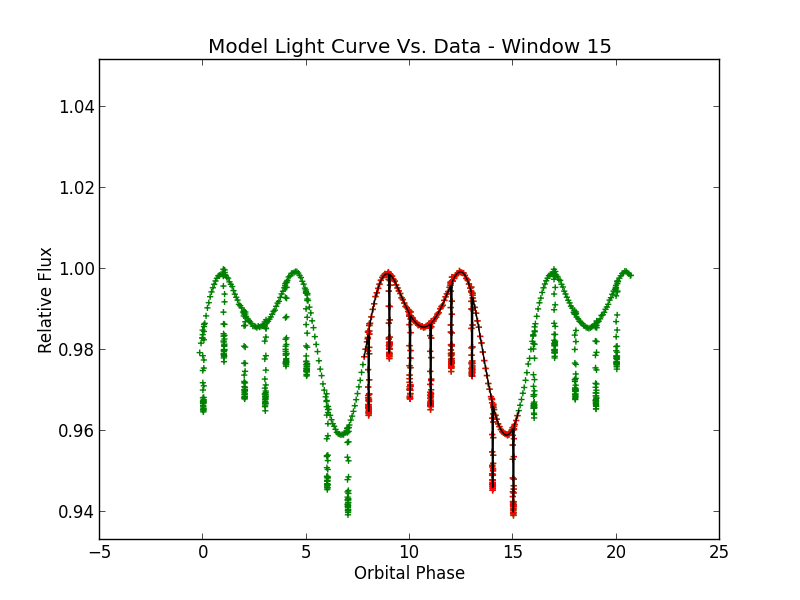
\includegraphics[width=.5\textwidth]{images/2b_2s/14_noise/model_fit_w15.png}
%	\caption{Typical light curve fit produced by the Eclipse Mapping code. The green points are the overall light curve data, the red points are the data for the current window, and the black line is the model fit for that window.}
%	\label{LC_Fit}
%\end{figure}